% What we have done (data preprocessing, getting the rhythmic instrument, retrieving the tokens, baseline using dadagp (GuitarCTRL))
\subsection{DadaGP token processing}
% --> Retrieving, cleaning, mapping DadaGP
% Rhythmic guitar detection (cite paper)

The DadaGP dataset provides token files containing information for all instruments in a score.
As we want to explore various conditioning combinations for tablature generation, we developed a function to extract tokens specific to selected instruments.
We considered several possible ways to perform this extraction: runnning DadaGP's token processing script for each instrument, or filtering the tokens from the complete token text file based on the instrument name.
Opening, parsing and looping on the GuitarPro file using pygp is needed for the DadaGP token processing script and is very time-consuming, much more than processing txt files.
We recall that DadaGP comprises 26,181 GuitarPro files. Using our algorithm it only took 5min30 to process all the files and generate the token files with the bass guitar tokens only.
To perform this operation, we leverage the fact that tokens of a given instrument start with the instrument name followed by a colon, e.g., \texttt{bass:} for the bass guitar.
However we must be careful not to miss the potential note effect tokens that are not instrument-specific, but come right after the token they are related to.
After extracting those tokens and the general tokens (metadata tokens and wait tokens),
we sum the potential consecutive wait tokens that were previously separated by notes from instruments that are no longer present.
An example of token extraction is shown in Figure~\ref{fig:token_list}.

\begin{figure}[!ht]
    \centering
    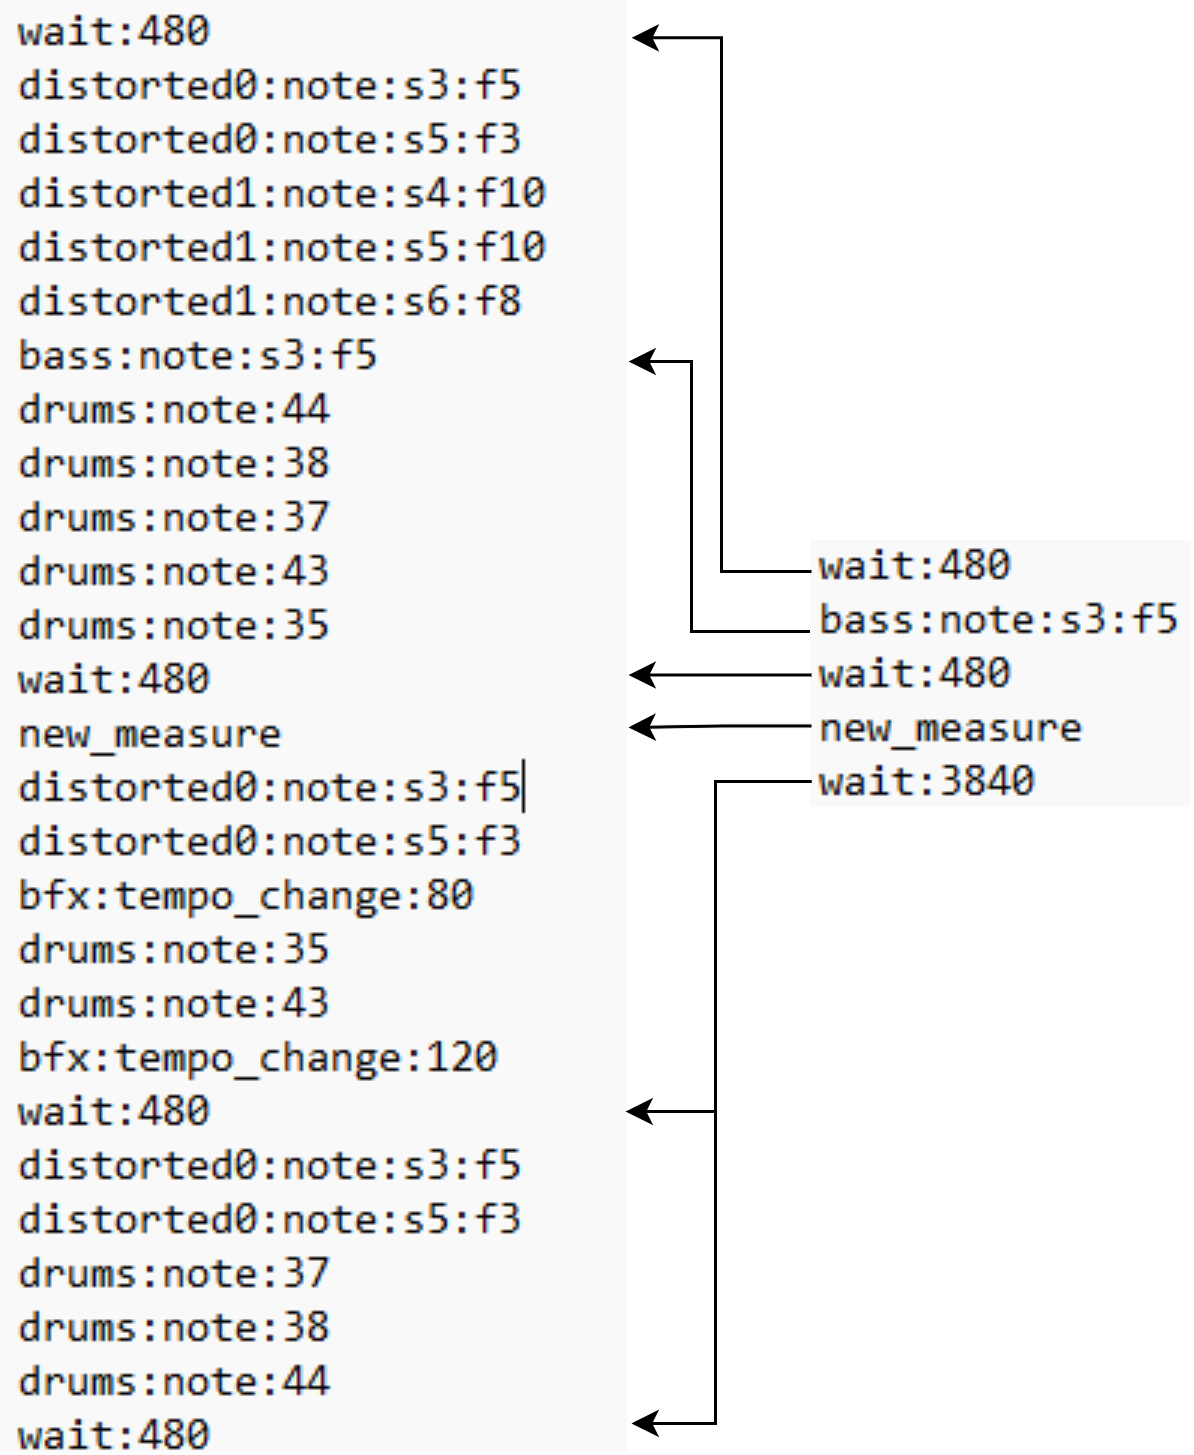
\includegraphics[width=.5\linewidth]{../images-figures/token_extraction.png}
    \caption{Example of an extraction of bass guitar token in The Strokes - Last Nite}
    \label{fig:token_extraction}
\end{figure}

An example of token extraction is shown in Figure~\ref{fig:token_extraction}.
This figure also shows the concatenation of wait tokens.
At the end of the song bass guitar stops playing before the other instruments. We can notice the different \texttt{wait:480} tokens that are summed up to a single \texttt{wait:3840} token.


\subsection{Rythmic guitar identification}

The algorithm we just presented allows us to extract tokens for any instrument in the DadaGP dataset.
We then focused on conditioning bass guitar tablature generation using the rhythmic guitar.
In typical rock band instrumentation, rhythmic guitars complement bass guitars with their repetitive chord patterns, providing harmonic and rhythmic structure at a higher pitch \cite{regnier_identification_2021}.
This characteristic makes them particularly relevant for conditioning bass generation tasks.

To identify rhythmic guitar parts in the DadaGP dataset, we implemented the method proposed by Régnier et al. \cite{regnier_identification_2021},
which uses features describing notes and chords at the bar level, along with corresponding tablatures.
Their model outputs a prediction between 0 and 1 for each bar. The closest to 1, the more likely the part is a lead on the bar, and the closest to 0, the more likely it is a rhythmic guitar part on the bar.
In their paper, they consider that a score below 0.5 correspond to a rhythmic guitar parts. We wanted to select and condition the generation on only one rhythmic guitar part, the "most" rhythmic.
Therefore, we applied the 0.5 threshold to the predictions and selected the part with the highest proportion of rhythmic bar over the course of the song.
Implementing this method required adapting their code to the DadaGP dataset.
Significant effort was spent mapping the identified rhythmic guitar parts to their respective names in the DadaGP files, as the dataset renames instruments, whereas the identification tool relies on GuitarPro part names.

\section{Baseline predictions}

With the preprocessed data, we began by establishing a baseline model for bass guitar tablature generation.
Initially, we utilized a pre-trained checkpoint from the DadaGP paper \cite{sarmento_dadagp_2021} without additional training.

To generate bass-specific outputs, we experimented with various prompts.
First, we provided a single bass guitar note as the initial token, however the model quickly incorporated tokens from other instruments.
This is an issue documented in the GuitarCTRL paper\cite{sarmento_gtr-ctrl_2023} where they used a metric called the UIP score (Unpromped Instrument Presence) to evaluate the model's ability to generate a specific combinations of instruments.
To constrain the output to bass tokens, we modified the logits of non-bass instruments by setting them to $-\infty$.

% FIGURE REPETITIVE GENERATION
\begin{figure}[!ht]
    \centering
    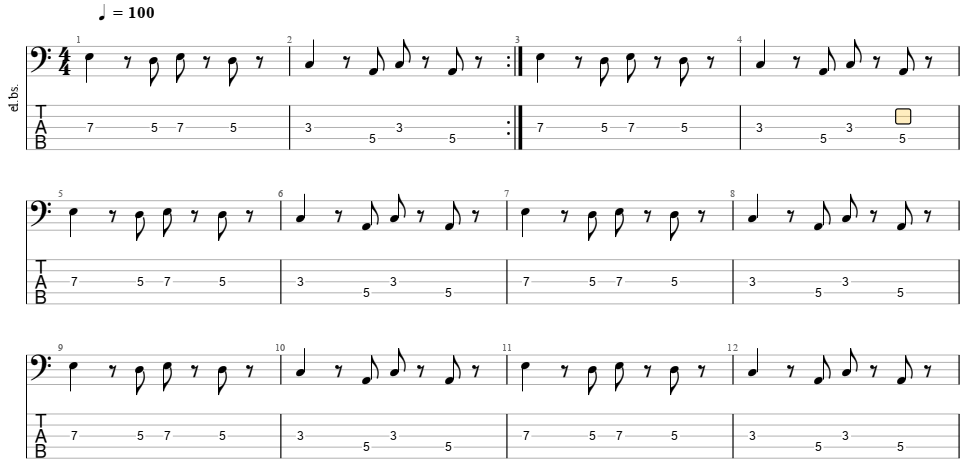
\includegraphics[width=.75\linewidth]{../images-figures/generated_bass_baseline.png}
    \caption{Example of a bass generation from the baseline model}
    \label{fig:repetitive_generation}
\end{figure}

An example of a bass tablature generated this way is shown in Figure~\ref{fig:repetitive_generation}.
While this forced the model to generate only bass tokens, the output quality was poor, featuring repetitive phrases, harmonically incorrect notes, or complete aberrations.
This was expected, as the model was not trained explicitly for bass only generation. 
Unfortunately, we cannot provide a quantitative evaluation of the generated tablatures, as we have not yet defined an evaluation metric.

\section{Workplan}
% Workplan (what we are going to do)

% DETAILS
Our next steps include:
\begin{enumerate}
    \item Propose an evaluation metric to quantify the quality of the generated tablatures.
    \item Understand the code of the model proposed by Makris et al. using their Github repository.
    \item Adapt the model to our task and our data.
    \item Generate predictions with conditional information from several combinations of instruments.
\end{enumerate}